\documentclass{article}[18pt]
\usepackage{../../../../format}
\lhead{Networks and Systems - Networks}


\begin{document}
\begin{center}
\underline{\huge Medium Access Control}
\end{center}
\section{The MAC Sublayer}
MAC is a layer responsible for determining who transmits next, i.e. who gets next access to the channel
\section{Key Issue}
We have a single physical layer medium for network communication, it may be a wire or it may be part of the wireless spectrum, but multiple connected nodes all want (or try) to use it at once to transmit/receive
\subsection{Why is this a problem}
If we nodes transmit at the same time on the transmission medium the transmissions interfere with each other and become corrupted
\section{Channel Allocation Problem}
Single channel is shared by several stations:
\begin{itemize}
	\item This channel can be allocated to only one transmitting user at a time
	\item Two different methods of channel allocation:
	\begin{itemize}
		\item Static channel allocation
		\item Dynamic channel allocation
	\end{itemize}
\end{itemize}
\section{Static Channel Allocations}
\begin{defin}[In Time Division Multiplexing]
Each user gets the entire transmission capacity for a fixed time interval
\end{defin}


\begin{defin}[In Frequency Division Multiplexing]
Each user gets a portion of the transmission capacity for the whole time
\end{defin}
\begin{center}
	\includegraphics[scale=0.7]{"TDM vs FDM"}
\end{center}
The limitations of static channel allocation
\begin{itemize}
	\item Works only for a fixed number of users
	\item Data traffic is very often bursty i.e. long time no data and for a short time high data
	\item If many users do not use their allocated channel capacity, most of the channels will be idle most of the time
\end{itemize}
\section{Dynamic Channel Allocations}
\begin{itemize}
	\item In this method, no user is assigned fixed frequency or fixed time slot
	\item All users are dynamically assigned frequency or time slot, depending upon the requirements of the user
	\item Many protocols have been defined to handle the access to shared link. They are organized in various different groups
	\begin{itemize}
		\item Random Access Protocols
		\begin{itemize}
			\item There is no rule that decides which station should send next
			\item If two stations transmit at the same time, there is a collision and the frames are lost
		\end{itemize}
		\item Controlled Access Protocols
		\item Limited Contention Protocols
		\item Channelization Protocols
	\end{itemize}
\end{itemize}
\section{Random Access Protocols}
\subsection{ALOHA}
\begin{itemize}
	\item Protocol developed for communication over radio link
	\item Collision occurs when two stations transmit simultaneously
\end{itemize}
\subsubsection{Pure ALOHA}
\begin{itemize}
	\item Stations transmit frames whenever they have data to send
	\item Collisions
	\begin{itemize}
		\item When two stations transmit simultaneously, there is a collision and frames are lost
		\item Whenever two frames try to occupy the channel at the same time, there is a collision and both the frames are lost
		\item If the first bit of a new frame overlaps with the last bit of a frame, both frames will be lost and both will have to be retransmitted
	\end{itemize}
\end{itemize}
\subsubsection{Slotted ALOHA}
\begin{itemize}
	\item In slotted ALOHA, the time is divided into frame-sized slots
	\item A station can send a frame only at the beginning of the slot, and only one frame is sent in each slot
	\item If any station is not able to place the frame onto the channel at the beginning of th slot, it has to wait until the next time slot
	\item There is a possibility of a collision if two stations try to send at the beginning of the same time slot
\end{itemize}
\subsection{Carrier Sense Multiple Access}
\begin{itemize}
	\item CSMA was developed to overcome the problems of ALOHA
	\item CSMA is based on the principle of "carrier sense"
	\begin{itemize}
		\item The station senses the carrier or channel before transmitting a frame
	\item I.e. station checks whether the channel is idle or busy - if busy then don't send
	\item Chances of collision reduce greatly if a station checks the channel before trying to use it
	\end{itemize}
	\item Chance of a collision still exists because of propagation delay
	\item A frame transmitted by one station takes some time to reach the other station
	\item In the meantime, other station may sense the channel to be idle and transmit a frame
	\item This results in a collision
	\item There are three types of CSMA protocols:
	\begin{itemize}
		\item 1-persistent (greedy) - sends as soon as idle
		\item Non-persistent - waits a random time then tries again
		\item p-persistent - sends with probability p when idle
	\end{itemize}
\end{itemize}
\subsubsection{1-Persistent CSMA}
\begin{itemize}
	\item In this method, station that wants to transmit data, continuously senses the channel to check whether the channel is idle or busy
	\item If the channel is busy, station waits until it becomes idle
	\item When the station detects an idle channel, it immediately transmits the frame
	\item When a collision occurs, the station waits a random amount of time and starts all over again
	\item This method has the highest chance of collision because two or more stations may find channel to be idle at the same time, and then will transmit their frames at the same time
\end{itemize}
\subsubsection{Non-Persistent CSMA}
\begin{itemize}
	\item A station that has a frame to send senses the channel
	\item If the channel is idle, it sends immediately
	\item If the channel is busy, it waits a random amount of time and then senses the channel again
	\item Reduces the chance of collision because the stations wait for a random amount of time
	\item Unlikely that two or more stations will wait for the same amount of time and will retransmit at the same time
	\item Introduces longer delays
\end{itemize}
\subsubsection{P-Persistent CSMA}
Used in slotted channels (slotted ALOHA)
\begin{itemize}
	\item Sense the channel
	\item If the channel is busy, then wait until the next time slot and start over
	\item If the channel is idle, then with probability p transmit with probability (1-p) defer until the next slot and start over
\end{itemize}
\subsection{CSMA/CD}
\begin{itemize}
	\item In \textbf{Carrier Sense Multiple Access with Collision Detection}, the station that sends its data on the channel continues to sense the channel while data is transmitted
	\item If collision is detected, the station aborts its transmission and waits for a random amount of time and sends its data again
	\item As soon as a collision is detected, the transmitting station releases a jam signal
	\item Jam signal alters all other stations. Stations are not supposed to transmitted immediately after the collision has occurred
	\item CSMA/CD improvement is to detect/abort collisions
	\begin{itemize}
		\item Reduced contention times improve performance
		\item A station who detects a collision immediately stops transmitting
		\item Afterwards it waits a random time and tries again
	\end{itemize}
\end{itemize}
\subsection{Comparing the protocols}
\begin{center}
	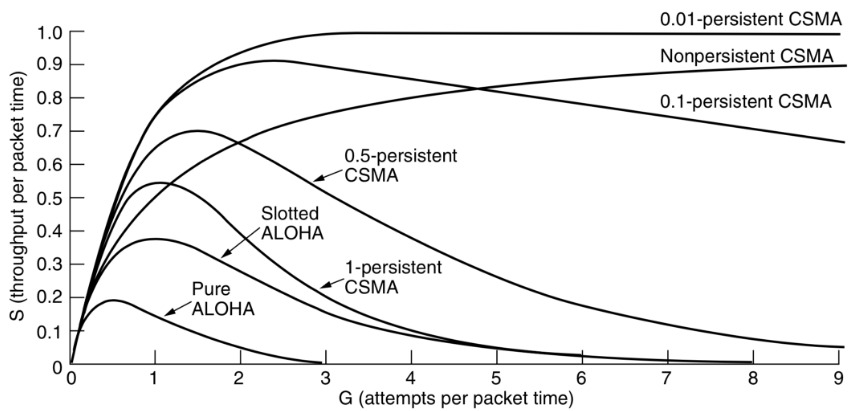
\includegraphics[scale=0.7]{Compare-Protocols}
\end{center}

\section{Controlled Access Protocols}
\begin{itemize}
	\item In these protocols, the stations consult each other to find which station has a right to send
	\item They are collision-free protocols
	\item A station cannot send unless it has been authorised by other stations
	\item There are three types of controlled access protocol
\end{itemize}
\subsection{Bitmap}
\begin{itemize}
	\item Before sending any data, all stations state if they have data
	\begin{itemize}
		\item Senders 0,1,2,...,n send their status one-by-one in order
		\item i.e. sender sets a bit in the contention slot if they have data
		\item Senders which announced they had data send in turn
		\item Repeat
	\end{itemize}
\end{itemize}
\subsection{Token passing}
Token sent round ring defines the sending order
\begin{itemize}
	\item Station with token may send a frame before passing
	\item Idea can be used without ring too, e.g. token bus
\end{itemize}
\subsection{Binary countdown}
Binary countdown improves on the bitmap protocol
\begin{itemize}
	\item Stations send their address in contention slot
	\item The channel ORs bits; stations give up when they send a 0 but see a 1
	\item Station that sees it full address is next to send
\end{itemize}



\end{document}